% !TEX root = ../om_ts_02.tex

\begin{frame} % название фрагмента

\videotitle{ETS(AAA)}

\end{frame}



\begin{frame}{ETS(AAA): план}
  \begin{itemize}[<+->]
    \item Добавляем сезонность в ETS!
    \item Прогнозы.
    \item Разложение на составляющие.
  \end{itemize}

\end{frame}


\begin{frame}
  \frametitle{Добавляем сезонность!}

  $y_t$ — наблюдаемый ряд;

  $\ell_t$ — тренд, очищенный ряд (\alert{единорог});

  $b_t$ — текущая скорость роста очищенного ряда (\alert{единорог});

  $s_t$ — сезонная составляющая (\alert{единорог});

  $u_t$ — случайная ошибка.

  \pause
  ETS(AAA):

  A — \alert{аддитивная} ошибка;

  A — \alert{аддитивный} тренд;

  A — \alert{аддитивная} сезонность. 

\end{frame}


% TODO: опечатка с u_t исправить на слайдах!
\begin{frame}
  \frametitle{ETS(AAA): уравнения}

  
  \[
    \begin{cases}
    y_t = \ell_{t-1} + b_{t-1} + \alert{s_{t-12}} + u_t; \\
    \ell_t = \ell_{t-1} + b_{t-1} + \alpha u_t, \text{ стартовое } \ell_0; \\
    u_t \sim \dN(0;\sigma^2) \text{ и независимы.} \\
    b_t = b_{t-1} + \beta u_t,\text{ стартовое } b_0; \\
    \alert{s_t = s_{t-12} + \gamma u_t}; \text{ стартовые } s_0, s_{-1}, \ldots, s_{-11}.
    \end{cases}
  \]

  \pause
  Параметры: $\alpha$, $\beta$, $\gamma$, $\sigma^2$, $\ell_0$, $b_0$, $s_0$, $s_{-1}$, \ldots, $s_{-11}$.

  \alert{Ограничение}: $s_0 + s_{-1} + \ldots + s_{-11} = 0$.
  

\end{frame}

\begin{frame}{ETS(AAA): сколько параметров?}

    Параметры: $\alpha$, $\beta$, $\gamma$, $\sigma^2$, $\ell_0$, $b_0$, $s_0$, $s_{-1}$, \ldots, $s_{-11}$.

    \alert{Ограничение}: $s_0 + s_{-1} + \ldots + s_{-11} = 0$.

    Сколько независимых параметров оцениваем?
    \pause

    Правильный ответ: 17.
    

\end{frame}

\begin{frame}
  \frametitle{ETS(AAA): прогнозируем}

  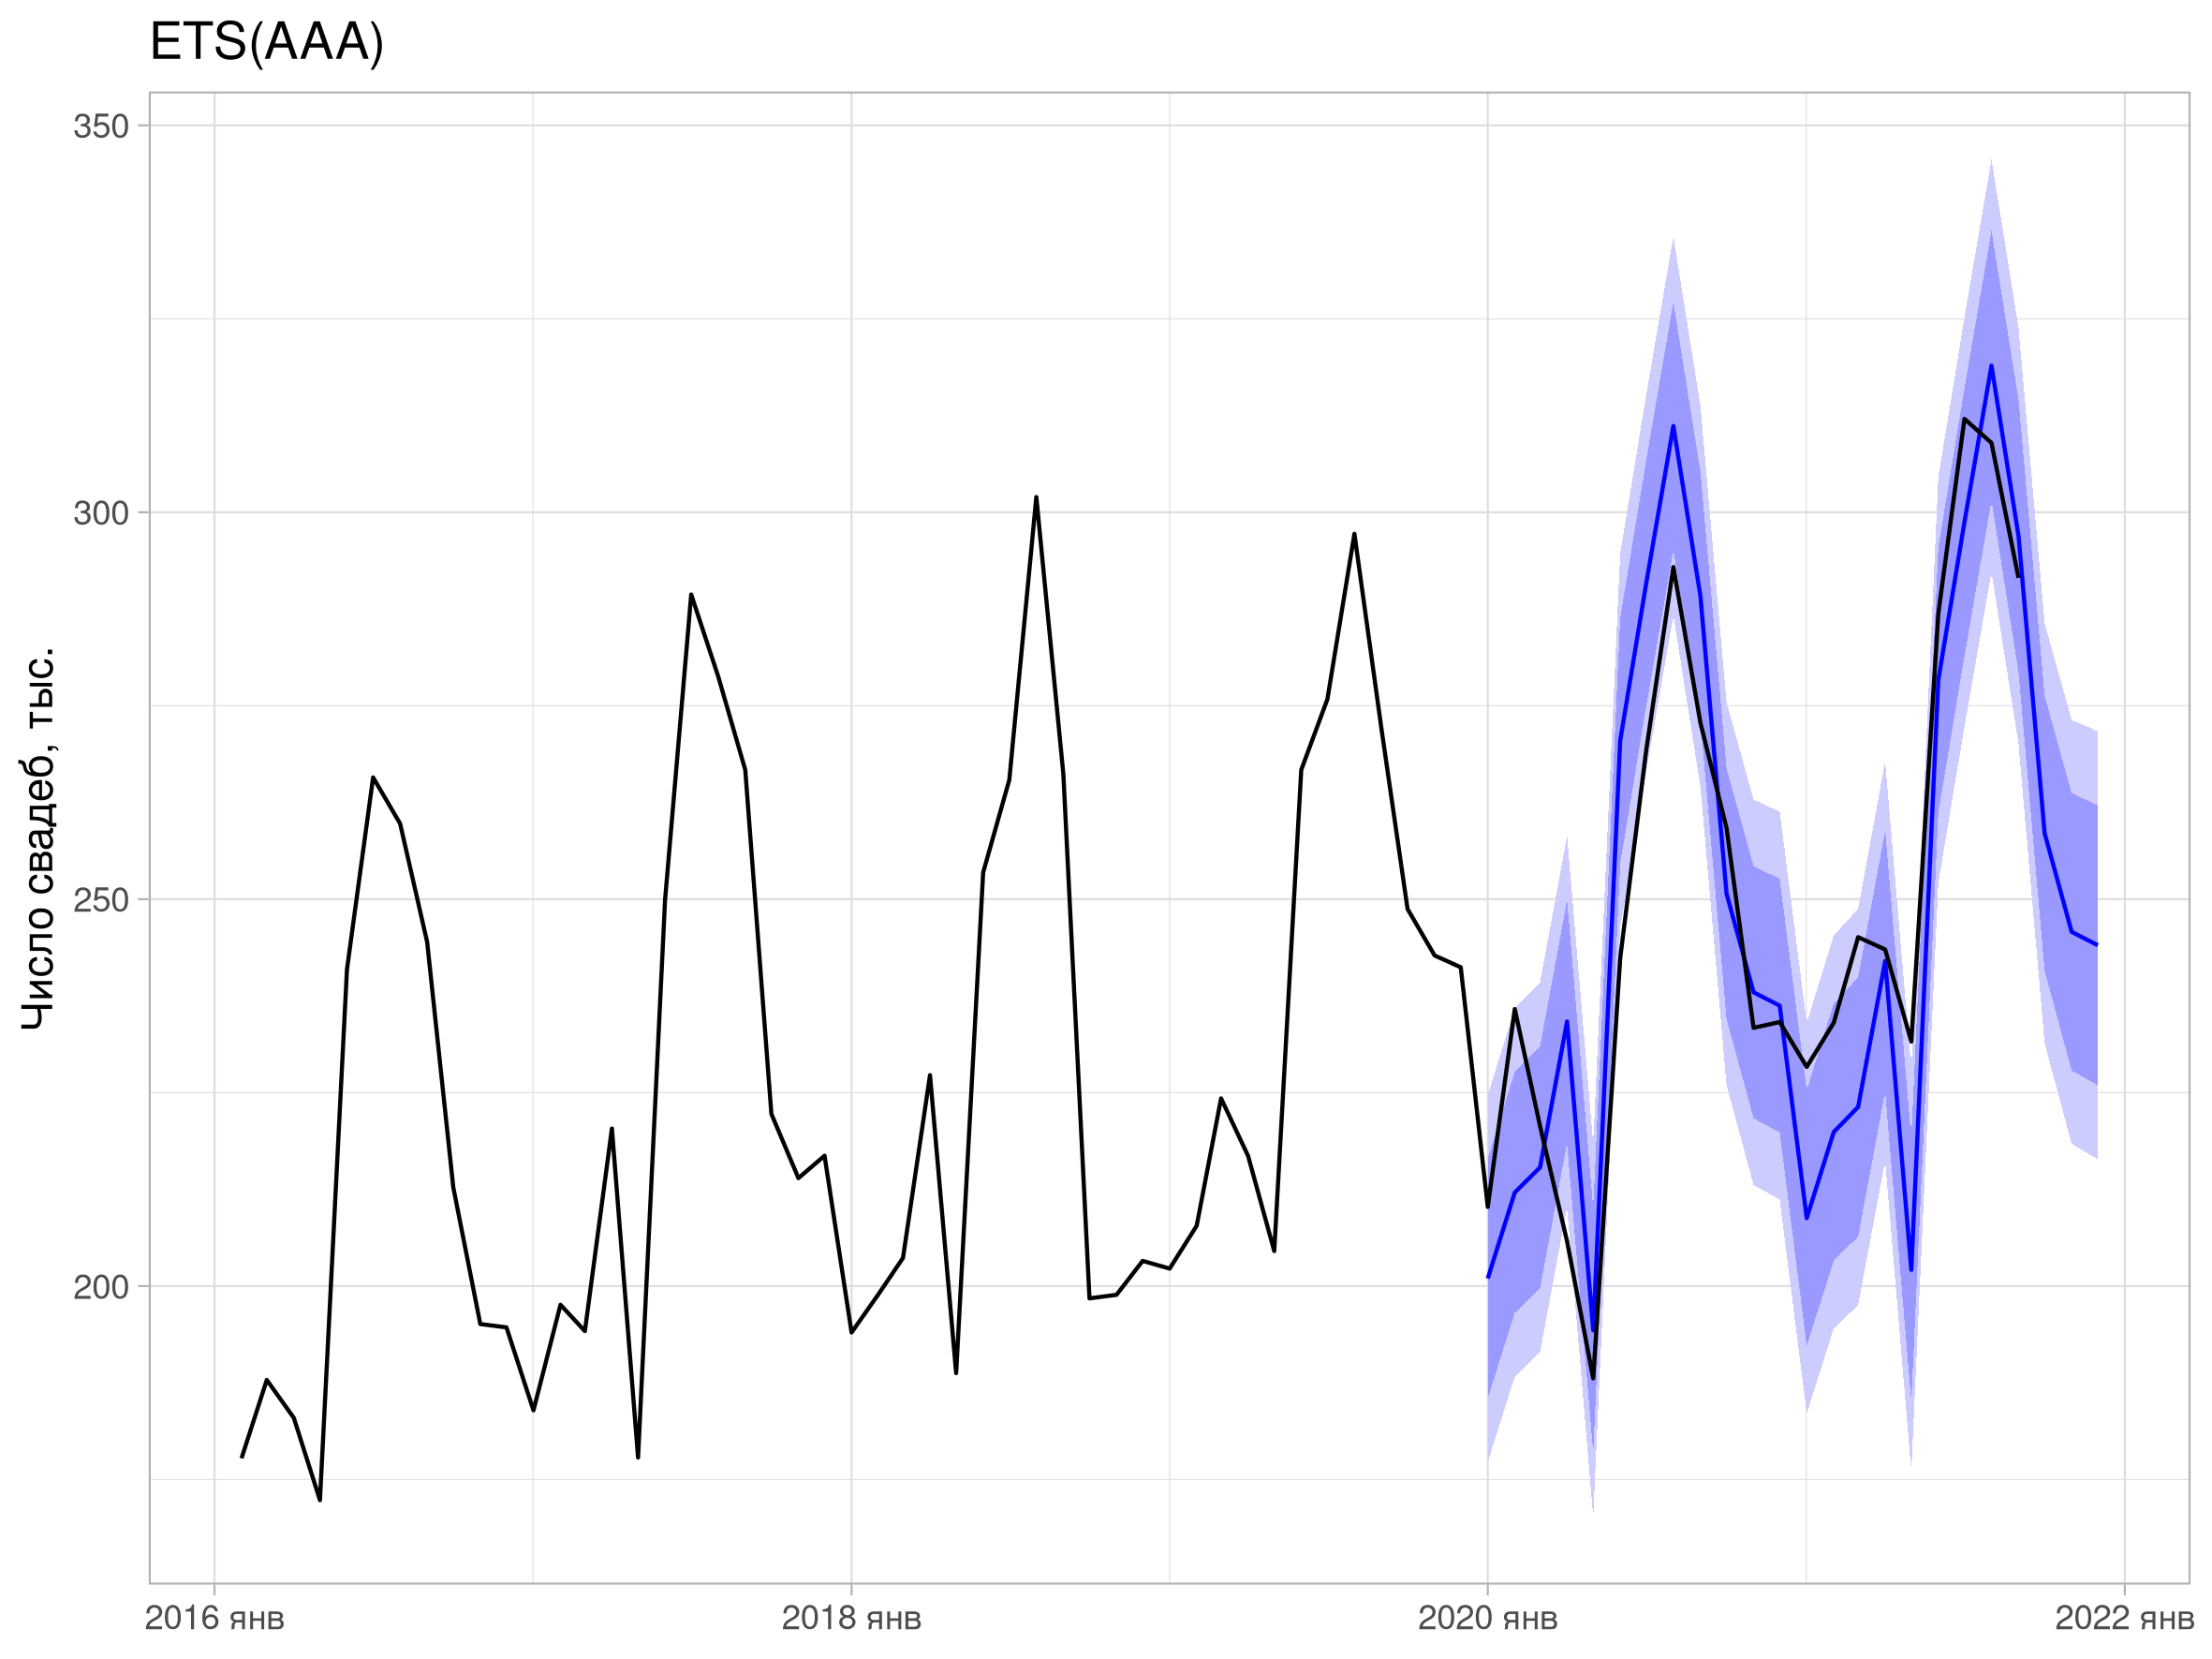
\includegraphics[width=\textwidth]{pictures/om_ts_02-076.png}


\end{frame}


\begin{frame}
  \frametitle{Прогноз на 1 шаг вперёд}

  \[
    \begin{cases}
     y_t = \ell_{t-1} + b_{t-1} + s_{t-12} + u_t; \\
    \ell_t = \ell_{t-1} + b_{t-1} + \alpha u_t, \text{ стартовое } \ell_0; \\
    u_t \sim \dN(0;\sigma^2) \text{ и независимы.} \\
    b_t = b_{t-1} + \beta u_t,\text{ стартовое } b_0; \\
    s_t = s_{t-12} + \gamma u_t
    \end{cases}
  \]
  \pause
\[
y_{T+1} = \ell_T + b_T + s_{T-11} + u_{T+1}  
\]
\pause
\[
  (y_{T+1} \mid \mathcal F_T) \sim \dN(\ell_T + b_T + s_{T-11}; \sigma^2)  
\]

\end{frame}


\begin{frame}
  \frametitle{Прогноз на 2 шага вперёд}

  \[
    \begin{cases}
        y_t = \ell_{t-1} + b_{t-1} + s_{t-12} + u_t; \\
       \ell_t = \ell_{t-1} + b_{t-1} + \alpha u_t, \text{ стартовое } \ell_0; \\
       u_t \sim \dN(0;\sigma^2) \text{ и независимы.} \\
       b_t = b_{t-1} + \beta u_t,\text{ стартовое } b_0; \\
       s_t = s_{t-12} + \gamma u_t
       \end{cases}
    \]
  \pause
  \begin{multline*}
    y_{T+2} = \ell_{T+1} + b_{T+1} + s_{T-10} + u_{T+2} = (\ell_T + b_T + \alpha u_{T+1}) +\\
    + (b_T + \beta u_{T+1}) + s_{T-10} + u_{T+2} 
  \end{multline*}
   \pause
  \[
  (y_{T+2} \mid \mathcal F_T) \sim \dN(\ell_T + 2b_T + s_{T-10}; \sigma^2((\alpha + \beta)^2 + 1))
  \]
  
\end{frame}


\begin{frame}
  \frametitle{Попутное разложение!}

  На выходе ETS(AAA):

  \alert{Оценки параметров}:  $\hat\alpha$, $\hat\beta$, $\hat\gamma$, $\hat\sigma^2$, $\hat\ell_0$, $\hat b_0$, 
  $\hat s_0$, $\hat s_{-1}$, \ldots, $\hat s_{-11}$.

  Ограничение: $\hat s_0 + \hat s_{-1} + \ldots + \hat s_{-11} = 0$.

  \pause 
  Оценённые \alert{значения составляющих}: $\hat \ell_t$, $\hat b_t$, $\hat s_t$.

  \pause 
  Автоматически получаем \alert{разложение}: $y_t = \hat \ell_t + \hat s_t + remainder_t$.

\end{frame}


\begin{frame}{ETS(AAA): итоги}

  \begin{itemize}[<+->]
    \item Ух, целых 17 параметров! 
    \item Наклон линии тренда и сезонность могут меняться.
    \item Автоматическое разложение на составляющие.
  \end{itemize}
\end{frame}



